\documentclass[USenglish,oneside,twocolumn]{article}
\usepackage{color}
\usepackage[hyphens]{url}
\usepackage{longtable}
\usepackage{graphicx}
\usepackage{enumitem}
\usepackage{pdfpages}
\usepackage{adjustbox}
\usepackage{subcaption}
%\usepackage{hyperref}

\usepackage[utf8]{inputenc}%(only for the pdftex engine)
%\RequirePackage[no-math]{fontspec}%(only for the luatex or the xetex engine)
\usepackage[big]{dgruyter_NEW}
 
\hyphenation{Isa-bela}

\DOI{foobar}

\cclogo{
\includegraphics{by-nc-nd.pdf}}

% Format a participant quotation.
\newcommand{\pquote}[2]{
\begin{quotation}
\noindent #1:~\textit{#2}
\end{quotation}
}
  
\begin{document}
   \author*[1]{Author 1}

  \author[2]{Author 2}

  \author[3]{Author 3}

  \author[4]{Author 4}

  \author[5]{Author 5}
  
  \author[6]{Author 6}

  \affil[1]{Affiliation of Author 1, E-mail: \mbox{author1@affiliation.edu}}
  \affil[2]{Affiliation of Author 2, E-mail: \mbox{author2@affiliation.edu}}
  \affil[3]{Affiliation of Author 3, E-mail: \mbox{author3@affiliation.edu}}
  \affil[4]{Affiliation of Author 4, E-mail: \mbox{author4@affiliation.edu}}
  \affil[5]{Affiliation of Author 5, E-mail: \mbox{author5@affiliation.edu}}
  \affil[6]{Affiliation of Author 6, E-mail: \mbox{author6@affiliation.edu}}
%  \author*[1]{Linda Lee}
%
%  \author[2]{David Fifield}
%
%  \author[3]{Nathan Malkin}
%
%  \author[4]{Ganesh Iyer}
%
%  \author[5]{Serge Egelman}
%  
%  \author[6]{David Wagner}
%
%  \affil[1]{University of California Berkeley, E-mail: \mbox{lnl@cs.berkeley.edu}}
%
%  \affil[2]{University of California Berkeley, E-mail: \mbox{fifield@cs.berkeley.edu}}
%
%  \affil[3]{University of California Berkeley, E-mail: \mbox{nmalkin@cs.berkeley.edu}}
%
%  \affil[4]{University of California Berkeley, E-mail: \mbox{ganesh.v@berkeley.edu}}
%  
%  \affil[5]{University of California Berkeley and International Computer Science Institute, E-mail: \mbox{egelman@cs.berkeley.edu}}
%   
%  \affil[6]{University of California Berkeley, E-mail: \mbox{daw@cs.berkeley.edu}}

  \title{\huge A Usability Evaluation of Tor Launcher}

  \runningtitle{A Usability Evaluation of Tor Launcher}

  %\subtitle{...}

  \begin{abstract}
{
We perform the first usability test on Tor Launcher, a graphical user interface (GUI) that all Tor Browser users must use to configure their initial connection to the Tor network. Users who do not require a proxy or a non-default bridge can usually connect to connect to the Tor network with the Tor Launcher GUI. However, user observations revealed that participants were intimidated by the tasks, unsure of what to do, and likely to get stuck configuring network components that they did not need. User testing showed that most users take more than 10 minutes to connect to Tor if the public relays are censored and half of the users cannot connect to Tor if the interface's hardcoded bridges are censored. We conclude with recommendations based on what we learned and by start a discussion on alternative 
approaches to bootstrap a connection to Tor. 
}
\end{abstract}
  \keywords{Usable Security, User Studies, Tor, Security, Censorship, Anonymity}
%  \classification[PACS]{}
 % \communicated{...}
 % \dedication{...}

  \journalname{Proceedings on Privacy Enhancing Technologies}
\DOI{Editor to enter DOI}
  \startpage{1}
  \received{..}
  \revised{..}
  \accepted{..}

  \journalyear{2015}
  \journalvolume{2015}
  \journalissue{2}

\maketitle

\section{Introduction}

Tor~\cite{dingledine2004tor} is an anonymity network that routes Internet traffic through a series of relays 
that make it difficult to observe the source and destination. 
Tor Browser~\cite{torbrowser} is a modified Firefox browser with a built-in Tor client that
is the recommended way to use Tor. Tor Launcher is a Tor Browser component that
starts, stops, and otherwise controls the underlying Tor processes.
Tor Launcher's graphical user interface (Figure~\ref{fig:old-interface}) asks the user to configure
bridges, pluggable transports, and proxies to make a connection to Tor (we refer to this graphical user interface as the ``configuration interface'' throughout this paper). This is the object of our study. 

Although Tor Browser was originally designed for Internet anonymity, many now use Tor Browser to circumvent Internet censorship. In fact, many countries block Tor relays specifically to prevent their citizens from circumventing censorship~\cite{winter2012great}. The configuration interface mainly exists so that people who face Internet censorship can configure bridges, transports, and proxies to connect to Tor, but all Tor Browser users must interact with it regardless of why they use Tor Browser.

Tor minimizes collecting user data. Therefore, Tor does not have data on how users interact with the configuration interface. While we agree that this is respectful to the users, we also believe that this data will be helpful to improve the usability of the configuration interface. Improving the usability of the configuration interface has the obvious benefit of helping more users connect to Tor. But this is also benefits the Tor Project (less help desk tickets) and other Tor users (an increase in overall users increases the anonymity set~\cite{dingledine2006anonymity}). 

We started our usability evaluation by inspecting the interface (section~\ref{sec:inspection}) and
running observing participants interact with it (section~\ref{sec:qualitative}). 
We opportunistically used the insights from our observations to make some changes (section~\ref{sec:design}).
Then we quantified how usable the interface was, and 
how much our changes helped save users time (section~\ref{sec:quantitative}).
Afterward, we gave some recommendations (section~\ref{sec:recommendations}), addressed
limitations of our evaluation (section~\ref{sec:limitations}), and framed our work in the context of existing work (section~\ref{sec:related}). \\

\noindent This paper contributes:
\smallskip
\begin{itemize}
\item an inspection of the Tor Launcher 5.0.3 interface
\item what users found challenging about the interface
\item measurements of how many users could connect
\item measurements of how long users took to connect
\item patterns seen in the users that failed to connect
\item recommendations to improve the interface
\end{itemize}

We hope that our work contributes to Tor Browser and is an informative case study of users interacting with anonymity and censorship circumvention tools. 

\section{Technical Background}
\label{sec:background}
This section discusses network components, when to configure them, and how they connect to Tor. 

\subsection{Proxies, Relays, Bridges, and Pluggable Transports} 

In this paper, the word ``proxy'' refers to a local, ordinary unobfuscated proxy such as a SOCKS or HTTP proxy. This is to maintain consistency with the wording in the configuration interface. Fig.~\ref{fig:topology} illustrates the interacting components. A proxy is technically an intermediary between clients and servers, so a single Tor relay, a bridge, the circuit of entry, middle, and guard relays, and local proxies can all can be considered a proxy. A user uses a proxy to bypass local firewalls. 

Tor relays are the routers in the Tor network. The Tor network is a group of routers that perform onion routing, a technique for anonymous communication over a computer network.  
Guard relays that serve as an entry node into the Tor network and receive packets from the user. Middle relays forward traffic from an entry relay to an exit relay, and provide an extra layer of encryption in the Tor network. Exit relays receive traffic from a middle relay, and direct the traffic to its intended destination. 
A user uses Tor Browser to connect to the Tor network, which indirectly connects to websites. 

Bridges are unlisted Tor relays that serve as an alternative entry node.
Bridges can be unlisted relays that behave similarly to a regular Tor relay,  
but most run a pluggable transport (referred to as ``transport'' for shorthand) that obfuscates traffic. 
Pre-configured bridges can be selected by ``Transport type,'' which refer to various
censorship circumvention technologies (``pluggable transports'').
Most transports rely on the secrecy of their static IP addresses for their effectiveness.
These include ``fte'' and ``fte-ipv6''~\cite{fte},
which disguise the Tor protocol as another protocol (such as HTTP), and
``obfs3''~\cite{obfs3}, ``obfs4''~\cite{obfs4}, and ``scramblesuit''~\cite{scramblesuit},
which encrypt or alter the Tor protocol to appear as random noise.
Other transports route traffic through other services and do not need secret IP address. 
``flashproxy''~\cite{flashproxy} connects through third party web browsers,
and the ``meek''~\cite{fifield2015blocking} options route traffic
through content delivery networks. Fig.~\ref{fig:old-bridge-combobox} shows the bridge and transport options at the time of the study. A user uses a bridge to connect to the Tor network while Tor relays or the Tor network protocol is being censored. 

\subsection{State and Corporate Censorship}
A local proxy is required to connect in certain managed networks (i.e. universities and corporations). This usually means that users cannot connect to the Internet at all without a proxy, including connecting to the Internet through Tor. The user must first successfully connect to the Internet through their proxy before trying to connect to a Tor relay or bridge. 

State level censors block access to the Tor network by blocking publicly listed Tor relays. Some also employ more sophisticated techniques such as deep packet inspection and protocol detection. This means that users can connect directly to (uncensored) websites, but Tor is blocked. The thoroughness of censorship is what requires different bridges and transports. 

\begin{figure}
\centering

\includegraphics{topology.pdf}
\caption{
The chain of components involved in connecting to a website over Tor.
Most users do not need a proxy;
only users who face a censor need a bridge.
In the diagram, ``Tor'' represents all three anonymizing hops through the Tor network.
We have shown the bridge as a separate component
because of the special role it plays.
When a bridge is used, it becomes the first Tor relay.
}
\label{fig:topology}
\end{figure}

\subsection{Connecting to Tor} 
A ``bridge line,'' a specifically formatted bridge specification that
includes its IP address, transport type, and other metadata 
officially configures Tor Browser to use bridges.
Users can do this more easily by choosing a 
a hard-coded option in the interface (see Figure~\ref{fig:old-bridge-combobox}) 
that select a group of bridges that use a particular transport.
For instance, choosing the hard-coded obfs3 option
configures a handful of bridges that use the obfs3 transport.
If the built-in bridges do not work, users can obtain bridge lines
through out-of-band channels~\cite{bridgedb}.

Configuring a proxy requires providing the proxy protocol, IP address, port, and additional optional fields. The user must locate and input this information. If the computer is already configured to use a proxy, the information can be found in other browsers. The interface tells users to ``check Internet settings in another browser'' if they are unsure of the proxy information. 

There are many valid configuration settings to connect to the Tor network.
A user who does not need a bridge or proxy can connect with a bridge, proxy, or both, provided that they are configured correctly. 

\begin{figure*}
\centering
\begin{subfigure}[b]{0.30\textwidth}
	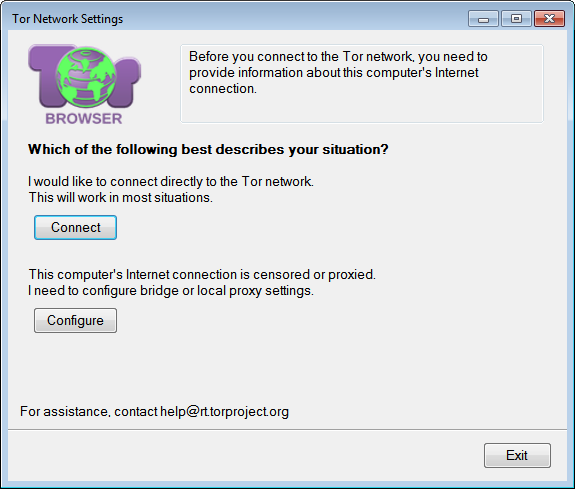
\includegraphics[width=\textwidth]{screenshots/OLD-first.png}
	\centering\captionsetup{width=1.5\linewidth}%
	\caption{The first screen (F). ``Connect'' connects directly to a public Tor relay unless bridges or proxies are configured.``Configure'' leads to the first bridge screen (Figure~\ref{fig:old-bridge}). }
	\label{fig:old-first}
\end{subfigure}
~~~~~~~~~~~~~~~~~~~~~~~~~
\begin{subfigure}[b]{0.30\textwidth}
	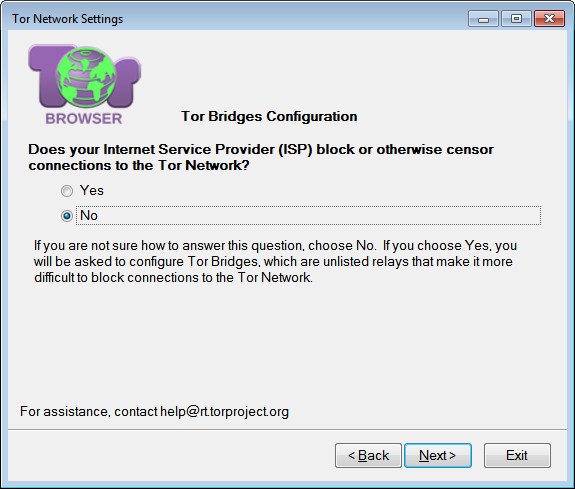
\includegraphics[width=\textwidth]{screenshots/OLD-bridges.png}
	\centering\captionsetup{width=1.5\linewidth}%
	\caption{The first bridge screen (B1). Answering yes directs users to a screen to configure bridges (Figure~\ref{fig:old-bridge-settings}). Answering no directs users to the proxy question screen (Figure~\ref{fig:old-proxy}).}
	\label{fig:old-bridge}
\end{subfigure}
~~~~~~~~~~
\begin{subfigure}[b]{0.30\textwidth}
	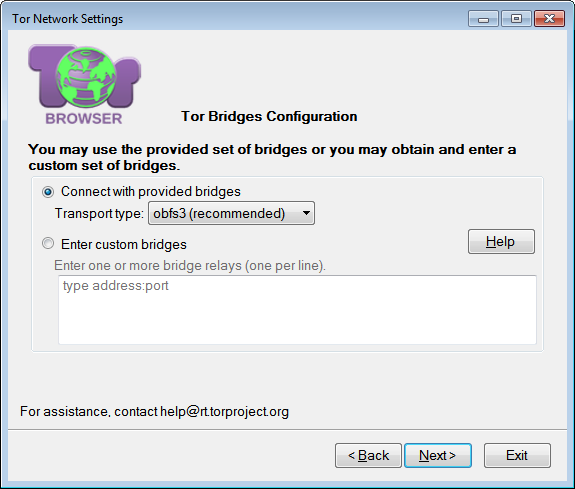
\includegraphics[width=\textwidth]{screenshots/OLD-bridgeSettings.png}
	\centering\captionsetup{width=1.5\linewidth}%
	\caption{The second bridge screen (B2). Users select a provided bridge or a custom one (bridges not hard coded into the interface). ``Help'' directs to bridge help screen (Figure ~\ref{fig:old-bridge-help}). }
	\label{fig:old-bridge-settings}
\end{subfigure}
~~~~~~~~~~~~~~~~~~~~~~~~~
\begin{subfigure}[b]{0.30\textwidth}
	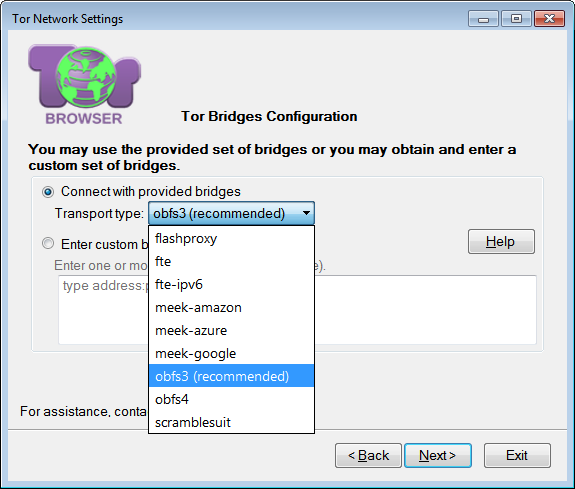
\includegraphics[width=\textwidth]{screenshots/OLD-bridgeSettings-combobox.png}
	\centering\captionsetup{width=1.5\linewidth}%
	\caption{The hardcoded bridges are listed alphabetically by the transport that they support. Each transport works differently, but their functions are not explained in the interface.}
	\label{fig:old-bridge-combobox}
\end{subfigure}
~~~~~~~~~~
\begin{subfigure}[b]{0.30\textwidth}
	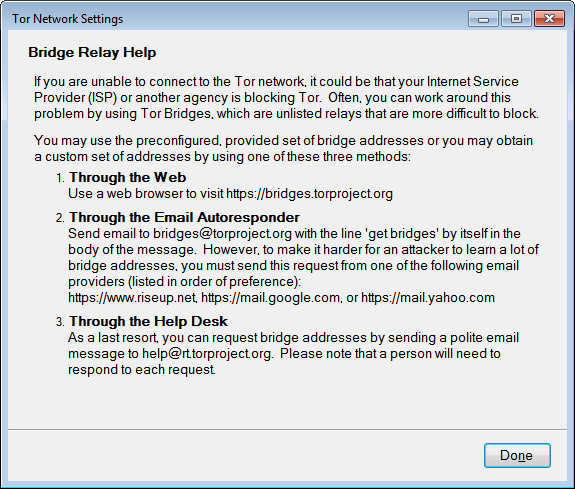
\includegraphics[width=\textwidth]{screenshots/OLD-bridgeHelp.png}
	\centering\captionsetup{width=1.5\linewidth}%
	\caption{The bridge help screen (BH) gives instructions for a custom bridge three different ways. ``Done'' redirects users back to the second bridge screen (Figure~\ref{fig:old-bridge-settings}).}
	\label{fig:old-bridge-help}
\end{subfigure}
~~~~~~~~~~~~~~~~~~~~~~~~~
\begin{subfigure}[b]{0.30\textwidth}
	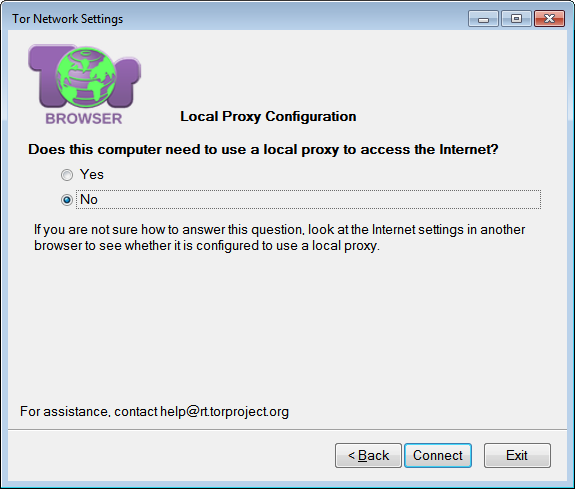
\includegraphics[width=\textwidth]{screenshots/OLD-proxy.png}
	\centering\captionsetup{width=1.5\linewidth}%
	\caption{The first proxy screen (P1). Answering yes to this question directs to the proxy settings screen (Figure ~\ref{fig:old-proxy-yes}). Answering no starts a connection to Tor.}
	\label{fig:old-proxy}
\end{subfigure}
~~~~~~~~~~
\begin{subfigure}[b]{0.30\textwidth}
	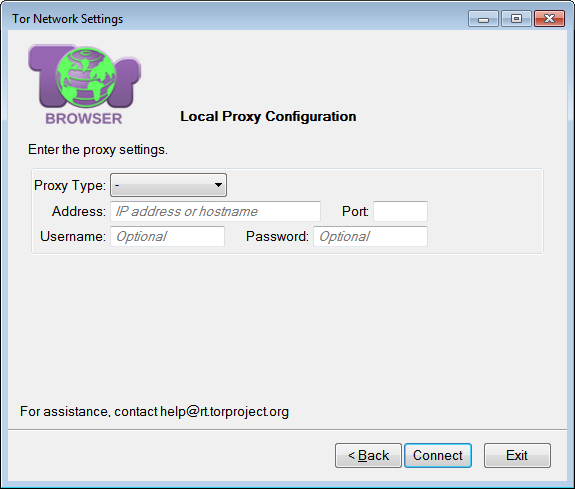
\includegraphics[width=\textwidth]{screenshots/OLD-proxyYES.png}
	\centering\captionsetup{width=1.5\linewidth}%
	\caption{The proxy settings screen (P2). Users configure a proxy by filling in the proxy's protocol, ip address, and port. ``Connect'' starts a connection to Tor with the interface settings.}
	\label{fig:old-proxy-yes}
\end{subfigure}
~~~~~~~~~~~~~~~~~~~~~~~~~
\begin{subfigure}[b]{0.30\textwidth}
	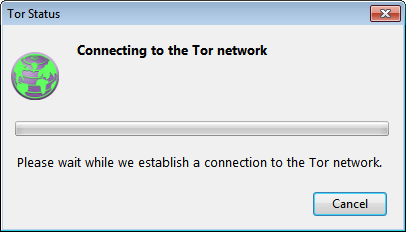
\includegraphics[width=\textwidth]{screenshots/OLD-progress.png}
	\centering\captionsetup{width=1.5\linewidth}%
	\caption{The progress bar (Pr). The bar fills up as log messages update the connection status. Warnings do not interruput this bar but an error replaces this window with an alert. }
	\label{fig:old-progress}
\end{subfigure}
\caption{
The Tor Browser 5.0.3 Tor Launcher GUI. Screens are in the order that they appear. 
}
\label{fig:old-interface}
\end{figure*} 

\section{Methodology} 
This section discusses how we performed our summative evaluation to determine the interface's effectiveness.

\subsection{Testing Pipeline} 
We performed a cognitive walkthrough~\cite{cognitive-walkthrough} of the interface by working tasks from the perspective of the user and assessing its learnability for new or infrequent users.

We then conducted qualitative and quantiative usability tests of the interface. We believed that both were necessary for a complete evaluation. Qualitative testing tells you {\it why or how} it is or is not usable, while quantitative testing tells you {\it how much} it is or is not usable. Five users is considered to be the maximum benefit-cost ratio for gaining insights~\cite{howmanyusers}, so we recruited five participants for each condition in our qualitative experiment. Twenty users is considered to be the minimum for statistically significant measurements~\cite{howmanyusers}, so we recruited twenty participants for each condition in our quantitative experiment.

We opportunistically used our observations from the qualitative study to design interface changes that would address common issues that our participants encountered. We also opportunistically used our quantitative testing setup to measure its usability with respect to the original interface. We found the process of identifying design principles, drafting design changes, and testing an alternative interface to be insightful and hope that this may be insightful to others as well. 

\subsection{Evaluation Metrics}
\label{sec:eval}
Usability measures users' abilities to complete tasks. We use the following industry-standard~\cite{albert2013measuring} metrics: \\

\begin{itemize}
\item {\bfseries Completion rate:}  percentage of users that connect to Tor in an experimental condition. 
\item {\bfseries Connection time:} time from Tor Browser startup to a successful connection to Tor. 
\item {\bfseries Configuration time:} time users spent in Tor Launcher configuring bridges and proxies, not counting time spent passively waiting.
\end{itemize}

Completion rate is the fundamental usability metric that measures if users can accomplish the task. We defined success as a binary metric that is true if a user connected to Tor and false if a user did not. 

Task time is a supplemental usability metric that measures user productivity during the task. We measured this in two ways. Connection time measures how long users took to connect to Tor, which includes time spent waiting for Tor to configure relays for the user. This can take up to a couple minutes and dominate the measurement. Configuration time measures the time users spent configuring bridges and proxies. 

\subsection{Experimental Setup}
\label{sec:environments}
We use versions of Tor Browser~5.0.3, 
the most recent stable release at the time~\cite{torbrowser-503}.
There were new releases during the experiments, but
we used the same version throughout to not introduce
confounding factors.

We simulated three environments of increasing severity in censorship (E1, E2, E3).
Table~\ref{tab:environments} summarizes them and explains what is required to connect to Tor. We chose to 
simulate environments for the stability and reproducibility of the 
experiment, as real censored networks are volatile and complex. 

\begin{table}[t]
\centering
\begin{tabular}{r c c c}
& E1 & E2 & E3 \\
% \noalign{\hrule}
websites blocked & X & X & X \\
public relays blocked & & X & X \\
default bridges blocked & & & X \\
\end{tabular}
\caption{
Summary of our simulated censorship environments.
E1 only requires users to connect directly;
E2 requires users to connect with a built-in bridge;
and E3 requires users to connect with a specific type of built-in bridge
or a custom bridge.
E2's blocking is a superset of E1's;
similarly E3's is a superset of E2's.
}
\label{tab:environments}
\end{table}

The simulated environments are not intended to imitate any particular country's censorship environment. Rather, they were designed to require particular network configurations
to connect to Tor. We believe this to be sufficient for the purpose of testing the configuration interface, since these environments require the user to take the interface paths we wanted to test. 

We conducted our studies at <redacted>, which only had Windows machines. 
So we used Windows Firewall rules to block IP addresses of public Tor relays (E2, E3) and default bridges (E3). 
and the Windows operating system hosts file to block websites by
mapping domain names to localhost (127.0.0.1) (E1, E2, E3). For all experiments, we blocked torproject.org and its subdomains to discourage downloading Tor Browser (as we had installed a specific version on the test computers) and wikipedia.org, cnn.com, and their subdomains (these were our simulated ``censored'' websites). 

\section{Usability Inspection}
\label{sec:inspection}
This section discusses our inspection of the configuration interface and the resulting observations.

\subsection{Procedure} 
Two researchers performed the cognitive walkthrough on the Tor Browser 5.0.3 Tor Launcher GUI, the most recent version deployed at the time (Figure~\ref{fig:old-interface}). We systematically tried actions from the perspective of a typical user, which we defined as a first time or infrequent user with almost no previous knowledge about network components involved in connecting to Tor.

We first examined each screen in the interface for tasks required, inputs taken, and consequences of possible actions. This was done to map all potential paths through the interface (Figure~\ref{fig:digraph}). We then stepped through each user path and recorded our observations. 

\subsection{Observations}
The interface did not suppose that a user has previous exposure to Tor. To help new users, it provided recommendations in the text and populated some options (such as bridges) with recommended options. However, the interface did require the user to figure out if Tor relays are blocked or if a proxy is required. And the interface did not discourage users from configuring components that are not necessary to connect to Tor. The proxy configuration has the potential for a lot of error, as there are a many free-form input fields. 

More generally, we suspected that new users or infrequent users would struggle to configure bridges and proxies. We doubted that users would have an understanding of how the Internet well enough to even explain how Tor relays, bridges, and proxies worked. Additionally, as mentioned previously, Tor relays, bridges, and proxies all allow indirect connections, and the difference in terminology can be confusing. The terminology of bridges and transports are also specific to Tor, and not other censorship circumvention software. 

We used the map of potential user paths (Figure~\ref{fig:digraph}) to design our simulated environments (section~\ref{sec:environments}).  We used our walkthrough observations as inspiration for drafting our post-experiment interview questions (Appendix~\ref{interview-questions}) for qualitative usability testing. 

\begin{figure*}
\centering
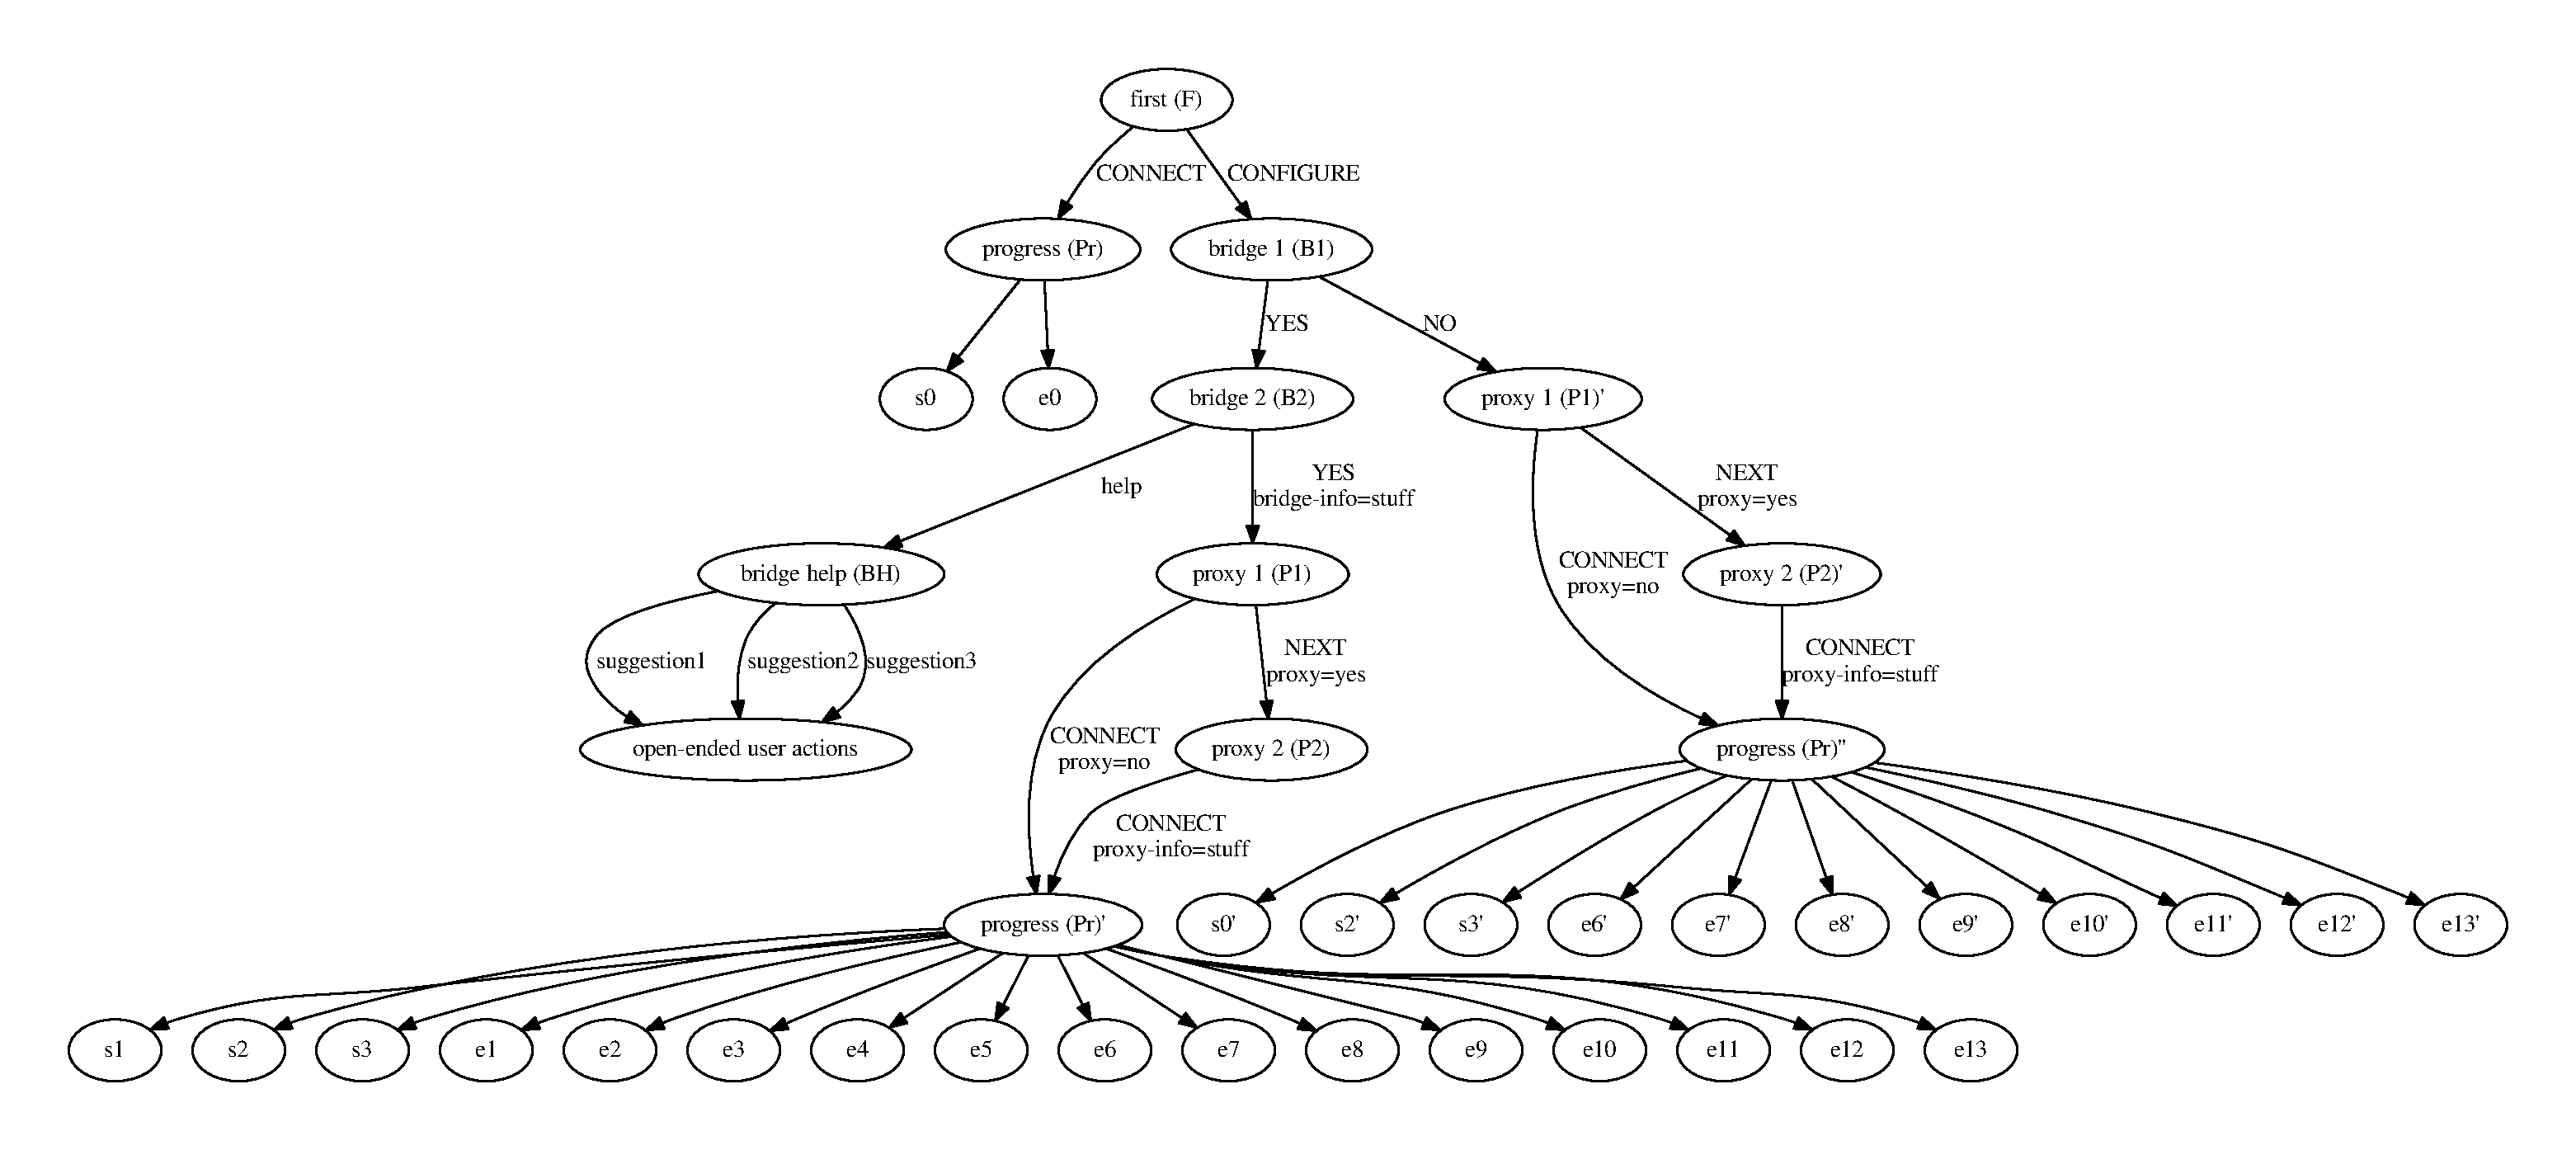
\includegraphics[width=\textwidth]{torconfig.pdf}
\caption{
A digraph illustrating the potential user paths through the interface. Non-leaf nodes are screens in the user interface (start, bridge 1, bridge 2, proxy 1, proxy 2, and progress). Leaf nodes are various end states (quit, success, or error). Transitions between these nodes denote user actions. For details of each end state, see Appendix~\ref{states}. 
}
\label{fig:digraph}
\end{figure*} 

\section{Qualitative Testing}
\label{sec:qualitative}
This section discusses our small-scale, qualitative usability experiment and resulting user insights. 

\subsection{Recruitment}
We recruited people from Craigslist using the recruitment text in Appendix~\ref{qualitative-recruitment}, which linked a prescreening survey that collected demographics (Appendix~\ref{qualitative-prescreening}). We pre-screened~\cite{screening} so that we could have a diversity of gender, age, technical expertise, use of security tools, and familiarity with Tor in a small participant pool. Of our 16 recruited participants, 50\% identified as male and 50\% identified as female. Ages ranged from 20 to~62 years ($\mu = 30.5$, $\sigma = 13.5$). One participant declined to report their age, so age calculations omit this participant's information. All of our users were highly educated, having at least some college education. We verified their self-reported familiarity with Tor Browser in-person to identify new users, and found that 12 were new users and 4 had previously used Tor Browser in some capacity.  

% gender: Male: 8/Female: 8
% education: At least some college 16
% ages: 22, 23, 34, 52, 25, 22, 29, 21, 25, didn't answer, 20, 20, 26, 24, 62, 52


We distributed participants evenly in number across experimental conditions:  5~in E1, 5~in E2, and 6~in E3. We ensured that each condition had a participant who had used Tor Browse before, and tried for some variation in gender, age, ``technical expertise,'' and ``use of security tools'' in each experimental condition as well. 

\subsection{Setup} 
We ran the experiment in a meeting room in <redacted building> at <redacted university>. The room had a desk and chair, where a monitor, keyboard, and a Windows computer were set up. On a clean computer, we manually downloaded and installed the necessary software for the experiment: Tor Browser 5.0.3 for testing, Chrome, Firefox, and Internet Explorer so that participants could browse the Internet in a another browser of their choice, and VLC to record the screen during the experiment. Before each participant entered the room, we ran a script on the computer that
set up one of the three simulated environments (E1, E2, or E3) and started recording the computer screen.  

\subsection{Procedure}
Three researchers ran the qualitative user tests. Each session had at least two researchers.  
We told the participant the purpose of the 
study, what data was collected, and any associated risks. 
Then they signed a consent form with this information in writing. 
Before the experiment, we clarified that they could stop at any time during the experiment with no negative consequences. 

We started by informing the participant of the simulated censorship environment (Appendix~\ref{qualitative-script}) and task. We explicitly stated that the they should use Tor to circumvent censorship. 
We instructed them to visit sample censored and uncensored websites
in a non-Tor browser to clarify that the Internet was functioning and
pointed out the Tor Browser shortcut on their desktop.

They were asked to complete a worksheet (Appendix~\ref{participant-worksheet}) that 
required answers from Wikipedia (censored) and CNN (uncensored).
We chose these websites because their likely familiarity~\ref{alexa}
would make the task seem less intimidating. They were given 45 minutes to complete the task. 
After instructions, researchers left to minimize interactions and watched a live feed of the participants' screen from another room.

After they completed the worksheet (or ran out of time),
we asked them general questions about their experience (Appendix~\ref{interview-questions}) and participant-specific questions to verify any hypotheses we had (e.g. ``the participant was selecting bridges at random''). We paid each participant~\$30 for their time. 

\subsection{Results} 

To see a summary of what each of our 16 participants did, see Appendix~\ref{summaries}. 

\subsection{Pain Points in Tor Launcher} 
\label{sec:pain-points}
We talk about the main challenges our participants faced during the experiment. 
Quotations were transcribed live during the follow-up interview.

The interface uses a technical and Tor-specific terms that are unfamiliar to an average user, such as the Tor network, internet service provider (ISP), local proxy, bridges, and transports. Participants found the interface confusing, and were often unable to answer the questions that were designed to guide them (Figures~\ref{fig:old-bridge} and~\ref{fig:old-proxy}) and did not know what to do to configure bridges and proxies (Figures~\ref{fig:old-bridge-combobox} and~\ref{fig:old-proxy-yes}).

%P3 in the repo, P3 in the paper
\pquote{P3}{``The vocabulary is really challenging, for someone not doing IT work.''}

%P13 in the repo, P7 in the paper 
\pquote{P7}{``I didn't know where to start. I didn't know what to do. [I] was just fiddling, to be honest with you... it was kind of confusing.''}

In addition to not knowing what to do, they did not understand the choices that they had to make. 

%P2 in the repo, P2 in the paper 
\pquote{P2}{``I don't know what any of those (points to list of transports) means. I don't know what that (points to proxy settings) means at all."}

%P8 in the repo, P10 in the paper
\pquote{P10}{``I have no clue what's the difference between flashproxy, fte, etc. And why do I need a custom bridge if there are options built in?''}

%P15 in the repo, but P12 in the paper
\pquote{P15}{``I didn't know if this computer had any proxy information. I wasn't able to find it if it did. I went to every browser and could not find what they were talking about. I googled how I would find that and couldn't seem to get good information. [I] couldn't find anything that said tools.''}

%P11 in the repo, P9 in the paper
\pquote{P9}{``I think you can only answer this question correctly if you know what a local proxy is.
Otherwise you have no chance... because looking at the Internet setting in another browser could be anything.''}

The progress bar had dependencies that made it update oddly. If progress bar reached a 90\% and failed, the progress bar will remain at 0\% on the next attempt until the progress surpassed 90\%. This made many assume that their subsequent attempts were wrong.

%P13 in the repo, P7 in the paper 
\pquote{P7}{``I was kind of doubting myself because everything was really slow.''}

%P16 in the repo, P13 in the paper
\pquote{P13}{``Put in a 30 second timeout! I don't know, maybe it takes longer than that...''}

%P1 in the repo, P15 in the paper
\pquote{P15}{``there doesn't seem to be any timeout on any of this stuff. Am I waiting long enough? Should I wait 5 minutes?''}

We have additional concerns on system visibility, error recovery, and user workload. Users cannot see their settings before or while they are connecting. This is only visible on the bridge and proxy screens. Participants did not know what to do after a connection failed. Users should be made aware of what to fix. Users do too much work (reading text, click throughs, choices) in this interface. We show an attempt to fix these issues in Section~\ref{sec:design}. 

\section{Design Changes}
\label{sec:design} 

We limited ourselves to design changes that do not require infrastructural changes. Figure~\ref{fig:new-interface} shows the results. 

\begin{figure*}
\centering
\begin{subfigure}[b]{0.30\textwidth}
	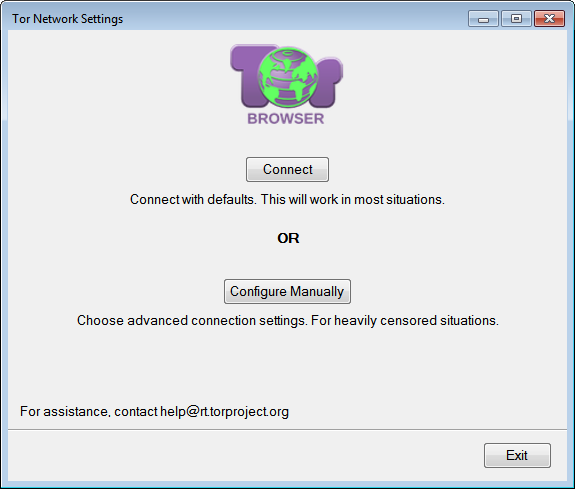
\includegraphics[width=\textwidth]{screenshots/NEW-first.png}
	\centering\captionsetup{width=1.5\linewidth}%
	\caption{The first screen (F). We reduced the text on the screen and clarified that configuration is for heavily censored environments. ``Configure'' leads to the proxy screen  (Figure~\ref{fig:new-proxy}.)}
	\label{fig:new-first}
\end{subfigure}
~~~~~~~~~~~~~~~~~~~~~~~~~
\begin{subfigure}[b]{0.30\textwidth}
	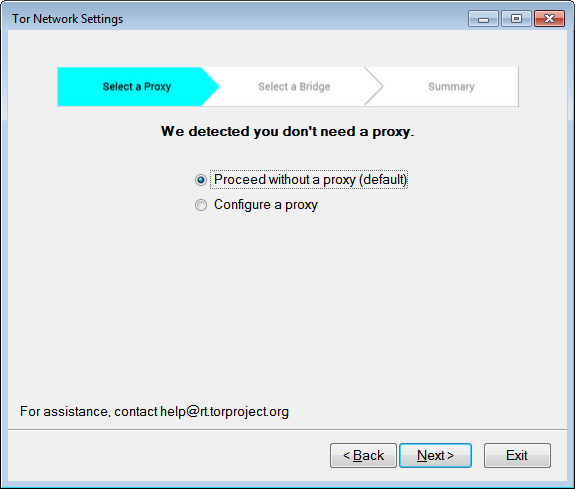
\includegraphics[width=\textwidth]{screenshots/NEW-proxyYES.png}
	\centering\captionsetup{width=1.5\linewidth}%
	\caption{The proxy screen (P). The interface locally detects if users need a proxy. If they need to configure one, proxy fields (same as Figure \ref{fig:old-proxy-yes}) are automatically populated.}
	\label{fig:new-proxy}
\end{subfigure}
~~~~~~~~~~
\begin{subfigure}[b]{0.30\textwidth}
	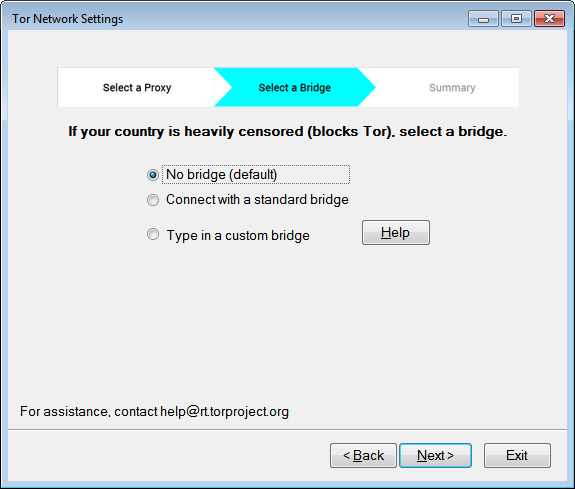
\includegraphics[width=\textwidth]{screenshots/NEW-bridgeSettings.png}
	\centering\captionsetup{width=1.5\linewidth}%
	\caption{The bridge screen (B). We give users the options to connect  without a bridge (the default choice) alongside the other options. We tell users to when to choose a bridge. }
	\label{fig:new-nobridge}
\end{subfigure}
~~~~~~~~~~~~~~~~~~~~~~~~~
\begin{subfigure}[b]{0.30\textwidth}
	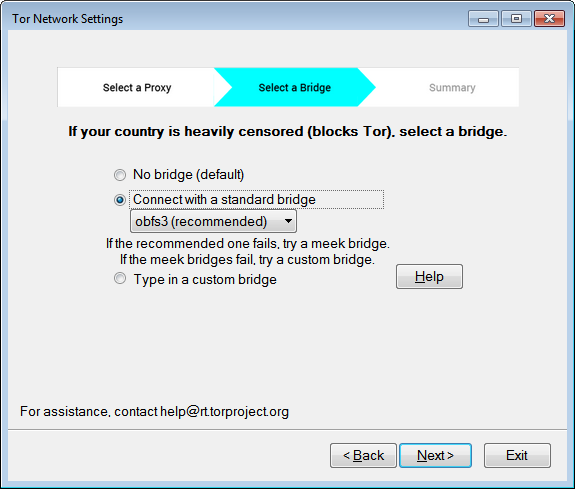
\includegraphics[width=\textwidth]{screenshots/NEW-bridgeSettings-default.png}
	\centering\captionsetup{width=1.5\linewidth}%
	\caption{We give a second bridge recommedation for the provided bridges. We hide the text field to input custom bridge information until they click the radio button to configure one.}
	\label{fig:new-bridge}
\end{subfigure}
~~~~~~~~~~
\begin{subfigure}[b]{0.30\textwidth}
	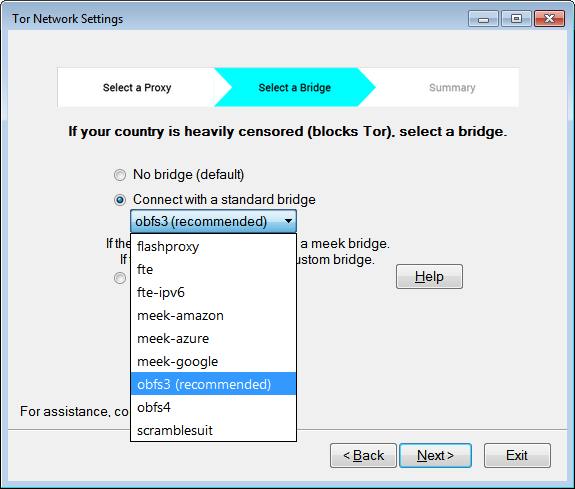
\includegraphics[width=\textwidth]{screenshots/NEW-bridgeSettings-combobox.png}
	\centering\captionsetup{width=1.5\linewidth}%
	\caption{The provided bridges and their supporting transports remains unchanged. This dropdown menu is the same as the bridge settings in the old interface (Figure~\ref{fig:old-bridge-combobox}).}
	\label{fig:new-bridge-combobox}
\end{subfigure}
~~~~~~~~~~~~~~~~~~~~~~~~~
\begin{subfigure}[b]{0.30\textwidth}
	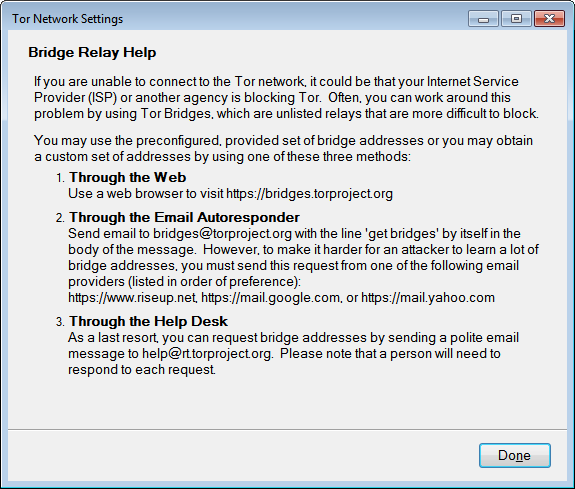
\includegraphics[width=\textwidth]{screenshots/NEW-bridgeHelp.png}
	\centering\captionsetup{width=1.5\linewidth}%
	\caption{The bridge help screen (BH). We did not make any changes to this page. This screen is idential to that in the old interface (Figure~\ref{fig:old-bridge-help}).}
	\label{fig:new-bridge-help}
\end{subfigure}
~~~~~~~~~~
\begin{subfigure}[b]{0.30\textwidth}
	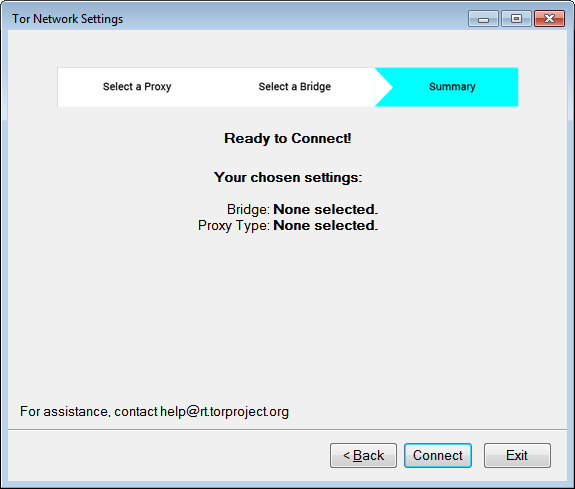
\includegraphics[width=\textwidth]{screenshots/NEW-summary.png}
	\centering\captionsetup{width=1.5\linewidth}%
	\caption{The summary screen (S). This screen shows users what they had configured in the interface. If they  configurued proxies or bridges, this summarizes their choices.}
	\label{fig:new-summary}
\end{subfigure}
~~~~~~~~~~~~~~~~~~~~~~~~~
\begin{subfigure}[b]{0.30\textwidth}
	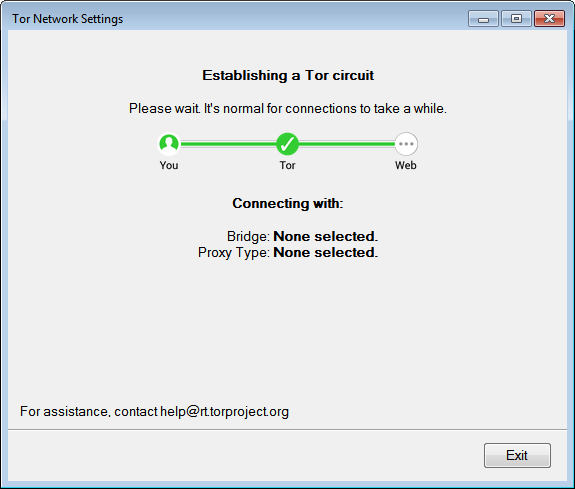
\includegraphics[width=\textwidth]{screenshots/NEW-progress.png}
	\centering\captionsetup{width=1.5\linewidth}%
	\caption{The progress bar (Pr). A checkpoint progress bar shows the status of each component in the connection (there are more checkpoints if bridges and proxies are configured).}
	\label{fig:new-progress}
\end{subfigure}
\caption{
A redesigned version of the Tor Browser 5.0.3 Tor Launcher GUI. Screens are in the order that they appear. 
}
\label{fig:new-interface}
\end{figure*} 

\subsection {Design Considerations} 

Changes were inspired by user observations and constrained by the following design considerations: 

\begin{itemize}
\item {\bfseries User consent}: Connecting to Tor requires consent since being revealed as using Tor can be dangerous. While we could help users by automating the configuration and connection process, taking on risk for the user without proper consent is not ethical. 

\item{\bfseries Active adversaries}: We could ask the user, "what country are you in?", "are you at risk?" or "do you know what you are doing?" to make decisions. While leveraging user input works well, third-party versions of Tor Browser will replicate the official version, but might steal the inputs to profile users. 

\item {\bfseries  Passive adversaries}: Assuming a sufficiently powerful network adversary (like governments), a failed, non-obfuscated attempt to connect to Tor will tell a passive eavesdropper that the user is connecting to Tor. We should allow users to leverage local information to reduce their risk.

\item{\bfseries  Maintenance constraints}: Network environments change all the time--what bridge was reachable in a country an hour ago might not be tomorrow. Keeping up with how and when each country censors Tor would require a lot of time. Even if we keep up with how and when each country censors Tor, we would need to push changes before any of the affected users connect to Tor, which is an unreasonable turnaround time.

\item{\bfseries  Financial constraints}: We could leverage harder-to-block meek relays connect people to Tor, then assign them something that would work afterward. But these relays cost thousands of dollars to run a month at their current capacity, and using them more would cost even more money.
\end{itemize}

It's possible that alternative changes could have been made, if we didn't treat these considerations as constraints. We start the discussion on methods that leverage user input and automation in Appendix~\ref{alternatives}. 

\subsection{Changes Made} 
To require less work, we eliminated the bridge and proxy questions from Figure~\ref{fig:old-bridge} and~\ref{fig:old-proxy} and simulated auto-detection for proxies by telling users that they did not need a proxy (this is feasible to implement with a local scan that does not leak information). 

To guide users, we label the configure button as an option heavily censored environments, tell users to configure a bridge if Tor is censored, and give a secondary bridge recommendation.

To help users understand, we added a summary screen displays the current bridge and proxy settings, switched proxy and bridge screens to put them in a topologically sequential order (Figure~\ref{fig:topology}), and added checklist indicators into the progress bar to that show if various components were reached.

\section{Quantitative Testing}
\label{sec:quantitative}
This section discusses our large-scale quantitative usability experiment and resulting user measurements. 

\subsection{Recruitment}
We recruited 65 participants from Craigslist and 59 participants from the <redacted lab> participant pool using text in Appendix~\ref{quantitative-recruitment}. <Redacted lab> encouraged the use of their participant pool, but we bargained to recruit participants from Craigslist to ensure a diverse set of participants. <Redacted lab>'s participant pool is mainly students and staff from <redacted institution>, even though anyone could join. 

We had 124 participants, but we filtered out 10 participants who did not complete the consent form correctly or did not interact with the instrumented interface. Of the 114, one participant did not report their demographics. We still use their experiment data. Of the 113, 44.2\% identified as male, 54.0\% identified as female, and 1.8\% identified as neither. Ages ranged from 18 to~68 years ($\mu = 28.2$, $\sigma = 12.3$). 84.1\% of our participants had at least a college education. We had about 20 in each interface and environment combination and ensured each condition had about half Craigslist recruited participants and half <redacted lab>  pool participants. 

\subsection{Setup}
We ran our experiment at <redacted lab>, an experimental social science laboratory for behavioral experiments. The testing room had 36 workstations with identical Windows~7 laptops. Side panels at each workstation to discouraged participants from looking at other screens. 
%Xlab~\cite{xlab}, the Experimental Social Science Laboratory at the University of California, Berkeley. 
The computers at <Redacted lab> use a system restore software to revert computers to a clean version at the beginning of each session. 

Before each session, we ran a script that downloaded Firefox, Chrome, IE, and VLC, set up one of the three simulated environments (E1, E2, or E3), and downloaded a version of Tor Browser 5.0.3 (original or our design), and started the computer screen recording. In contrast to the previous test, the Tor Browser 5.0.3 was instrumented to log user interactions with it (clicks, selects, transitions, etc.). Each computer was manually assigned one of the six interface--environment combinations in a way that evenly distributed experimental conditions throughout the room.

\subsection{Procedure}
We assigned participants  to a simulated censorship environment combination at random by being assigning them to a computer at random. We told the participants the purpose of the study, what data was collected, and any associated risks. Then they signed a consent form with this information in writing. Before the experiment, we clarified that they could stop at any time during the experiment with no negative consequences. 

We started by informing participants of the simulated censorship environment, giving them their worksheet,  informing them that Tor browser is necessary to circumvent censorship, and pointing out that Tor is installed for them on the computer (Appendix~\ref{quantitative-script}). They were asked to complete a worksheet that requires an answer from a censored site (Wikipedia) and explicitly reminds users to use Tor to do so (Appendix~\ref{summative-worksheet}). We reminded them to not show personal information since we are recording their screens, answered any questions, then gave them 40 minutes to complete the task. 

After instructions, researchers maintained minimal interactions with the participants, only answering logistical questions. Afterward, we administered an exit survey to collect demographics (Appendix~\ref{quantitative-exit-survey}). We paid each participant \$30 for their time. 

\subsection{Results} 
We summarize what our participants did below.  Table~\ref{table:participant-summary} gives an overview of the results and Figure~\ref{fig:all-participant-edges} summarizes all participants' paths during the experiment. In this section, we use OLD to refer to the deployed Tor Browser 5.0.3 Tor Launcher GUI (Figure~\ref{fig:old-interface}) and NEW to refer to our redesigned version (Figure~\ref{fig:new-interface}).

\label{all-participant-edges} 
\begin{figure*}
\centering
% This is a manually edited version of the automatically generated
% all-participant-edges graphic. It is edited to have better scale labels for
% the treatments.
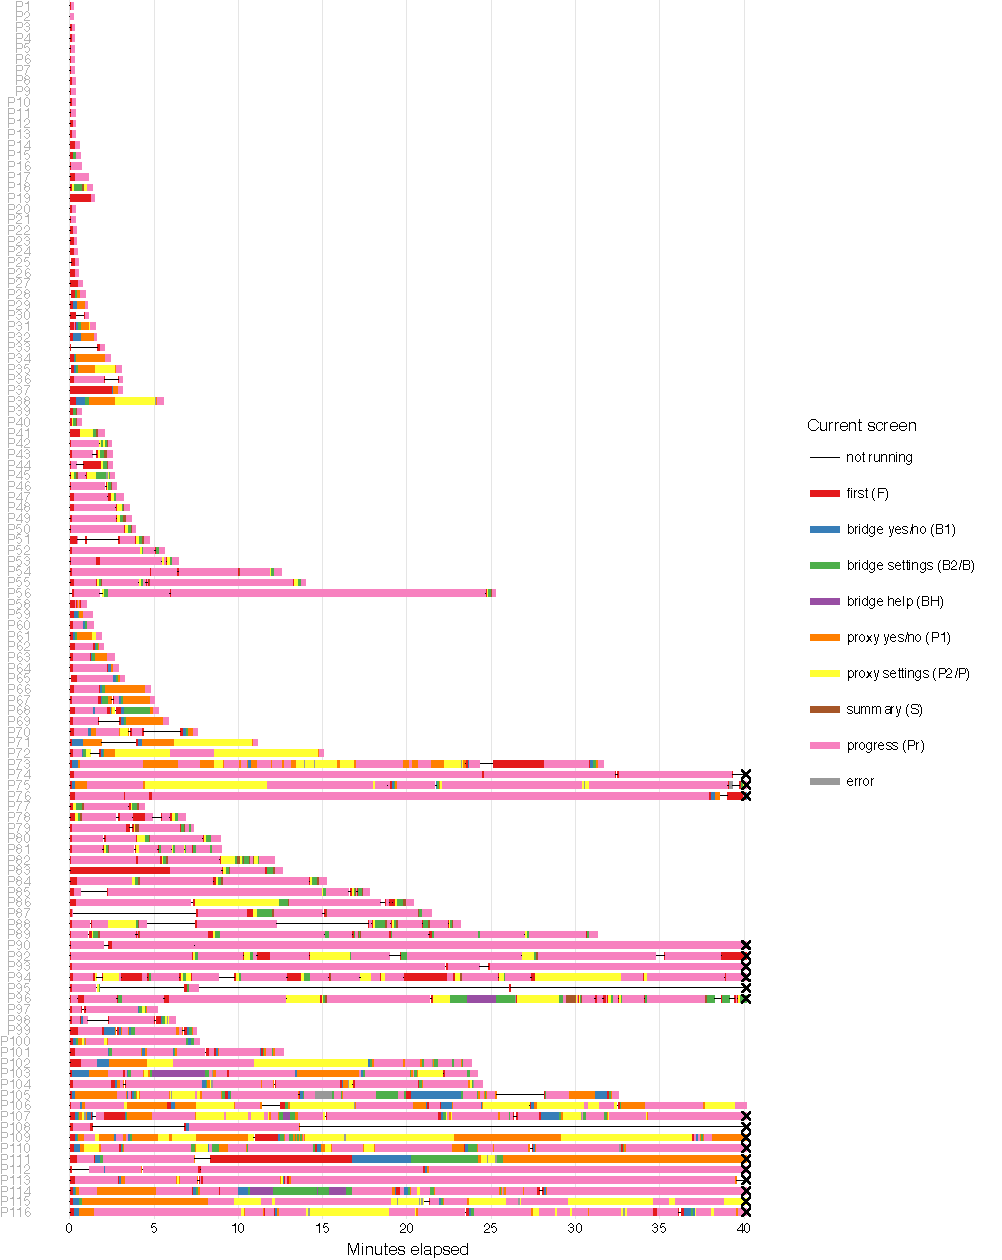
\includegraphics{all-participant-edges}
\caption{
A summary of our valid participants' paths through the interface.
The length of the bars show the total time taken to complete the task,
except for those we cut off after approximately 40 minutes.
Different colors indicate which screen they were on during the experiment.
If participants were doing other things (i.e. searching for help in another browser)
while off-focus, this time still counts as spending time in that off-focus window. 
``Not running'' are times when Tor Launcher was closed (
i.e. restarting the application).}
\label{fig:all-participant-edges}
\end{figure*}

\subsubsection{Completion Rate} 

\begin{table}[t]
\centering
\begin{tabular}{l r r r r r}
& \multicolumn{2}{r}{completion rate} & \multicolumn{1}{r}{connection} & \multicolumn{1}{r}{configuration} \\
& \multicolumn{2}{r}{(at 40min 8s)} & \multicolumn{1}{r}{time (med)} & \multicolumn{1}{r}{time (med)} \\
\noalign{\hrule}
E1-NEW & 19/19 & 100\% & 0:20 & 0:06 \\
E1-OLD & 19/19 & 100\% & 1:01 & 0:24 \\
E2-NEW & 18/18 & 100\% & 3:22 & 0:40 \\
E2-OLD & 16/19 & 84\% & 5:00 & 2:04 \\
E3-NEW & 13/19 & 68\% & 20:25 & 1:56 \\
E3-OLD & 10/20 & 50\% & 40:08 & 9:09 \\
\end{tabular}
\caption{
An overview of the results of the experiment. Those who
failed to connect were assigned the maximum time of 40:08, 
the maximum time a participant took to finish the task.
}
\label{table:participant-summary}
\end{table}

%table
\begin{table}[t]
\centering
% Do not edit this file. Edit attempts.R instead.
\begin{tabular}{r c c c c c c}
& \rotatebox{90}{E1-NEW} & \rotatebox{90}{E1-OLD} & \rotatebox{90}{E2-NEW} & \rotatebox{90}{E2-OLD} & \rotatebox{90}{E3-NEW} & \rotatebox{90}{E3-OLD} \\
no bridge, no proxy & 17 & 13 &  &  &  &  \\
obfs3, no proxy & 2 & 6 & 18 & 16 &  &  \\
meek-amazon, no proxy &  &  &  &  & 7 & 4 \\
meek-google, no proxy &  &  &  &  & 5 & 4 \\
meek-azure, no proxy &  &  &  &  & 1 & 1 \\
no bridge, 3rd-party proxy &  &  &  &  &  & 1 \\
DNF (did not finish) &  &  &  & 3 & 6 & 10 \\
\end{tabular}

\caption{
Network components that led to the first successful bootstrap
in each condition.
Most successful E1 participants used a direct connection,
but a few optionally used an obfs3 bridge.
All successful E2 participants used 
an obfs3 bridge (the recommended option)---none used 
flashproxy, fte, fte-ipv6, obfs4, or scramblesuit bridges to connect. 
Most successful E3 participants
used meek bridges, disfavoring meek-azure.
One E3 participant succeeded in an unexpected way
by using an open proxy and configuring it to bypass our 
simulated environment.
}
\label{tab:attempts-bridge-proxy}
\end{table}

%overview
Completion rate was defined as the percentage of users that eventually connected to Tor. Table~\ref{table:participant-summary} summarizes the completion rates and Table~\ref{tab:attempts-bridge-proxy} shows the configuration for users' first successful connection. We only considered the first successful configuration, as some curious participants tried others after completing their task. 

% failure observations
17\% (19 of 114) of participants were not able to successfully connect to Tor. Five (P73, P75, P89, P91, P106, P110) tried a direct connection. When that failed, they assumed there was something wrong with their computer, network settings, or the Tor network and never tried to configure bridges or proxies. Five (P74, P92, P105, P107, P113) users who need a bridge assumed that they needed a proxy to connect to Tor. We believe this may be due to the fact that the OLD interface defaults to showing users the proxy page (because it is the one before the progress screen) when a connection fails. Five (P90, P93, P108, P111, P114) users who needed a meek or custom bridge tried the suggested bridge (obfs3), but didn't know what to do when that failed. Two (P94, P109) users who needed a meek or custom bridge tried to get custom bridges but failed to format their email content correctly to get a response from the bridges autoresponder. We suspect that they would have succeeded if they had gotten a response.

%success rate and version
Our interface changes did {\it not} have a significant impact on completion rates (Pearson's Chi-squared; $\chi^2 = 2.808$, $\mbox{df} = 2$, $p = 0.094$). That is, the slight differences in completion rates between E1-NEW vs E1-OLD, E2-NEW vs E2-OLD and E3-NEW vs E3-OLD are likely due to random chance.

%using http://www.socscistatistics.com/tests/chisquare/Default2.aspx
% OLD VS NEW: The chi-square statistic is 2.8079. The p-value is .093802.
% E1-old vs E1-new: no valid calculation  since it's the exact same ratio (19 succeeded, 0 failed) 
% E2-old vs E2-new: The chi-square statistic is 3.0929. The p-value is .078636.
% E3-old vs e3-new: The chi-square statistic is 1.3666. The p-value is .242403.

\subsubsection{Connection time} 
Connection time is the time from Tor Browser startup to the first successful Tor bootstrap. Non-finishing participants are assigned the maximum experiment time of 40:08. Table~\ref{table:participant-summary} summarizes the median times while Figure~\ref{fig:time_to_success_clamped} shows their distribution. Figure~\ref{fig:time_to_success_ecdf} shows the cumulative success rates over time. 

%time observations (how long people took)
The simulated censorship environment, and therefore, the difficulty of the configuration, was the most determining factor for connection time (Kruskal--Wallis $\chi^2 = 80.5$, $\mbox{df} = 2$, $p < 10^{-15}$). Participants in E2 took longer to connect than participants in E1, and participants in E3 took the longest to connect.

%time to success and version
Our interface changes had a significant impact in reducing connection time (one-tailed Mann--Whitney; $ Z = -1.84$, $p = 0.0328$, $r= 0.172$). That is, the differences in mean connection times in E1-NEW vs E1-OLD and E2-NEW vs E2-OLD and E3-NEW vs E3-OLD is likely not due to random chance. We used a one-tailed Mann--Whitney test because the distribution of completion times were 1) right-censored at 40 minutes (experiment duration) and 2) non-normal and heavily right tailed (failures were assigned a time of 40 minutes). 

\begin{figure}[t]
\centering
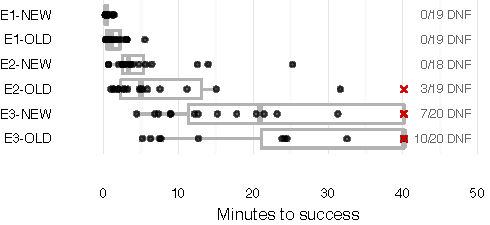
\includegraphics{time_to_success_clamped}
\caption{
Participants in E2 and E3 took a long time to connect.
The ``DNF'' (did not finish) shows how many of participants 
did not finish; they were assigned the maximum time of 40:08.}
\label{fig:time_to_success_clamped}
\end{figure}

\begin{figure}[t]
\centering
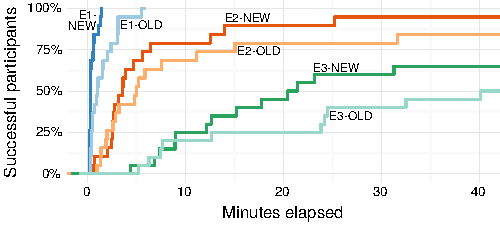
\includegraphics{time_to_success_ecdf}
%../experiment/processing/time_to_success_ecdf.tex
\caption{
Cumulative success rates over time. The longer the time went on, participants were less likely to succeed. 
}
\label{fig:time_to_success_ecdf}
\end{figure}


\subsubsection{Configuration Time} 
Configuration is defined as the completion time minus {\it any} time spent on the progress screen.Table~\ref{table:participant-summary} shows the median times and Figure~\ref{fig:time_to_success_active_clamped} shows their distribution. Table~\ref{table:median_time} shows where participants spent their time.  

\begin{table}[t]
\centering
\begin{tabular}{l r r r r}
& First & Proxy & Bridge & Progress \\
\noalign{\hrule}
E1-NEW & 28\% & 0\% & 0\% & 60\% \\
E1-OLD & 30\% & 0\% & 0\% & 29\% \\
E2-NEW & 6\% & 5\% & 6\% & 78\% \\
E2-OLD & 7\% & 18\% & 8\% & 45\% \\
E3-NEW & 3\% & 5\% & 5\% & 77\% \\
E3-OLD & 2\% & 12\% & 6\% & 64\% \\
\end{tabular}

\caption{
The median percent of time spent on each screen, aggregated over participants in each experimental condition. }
\label{table:median_time}
\end{table}

\begin{figure}[t]
\centering
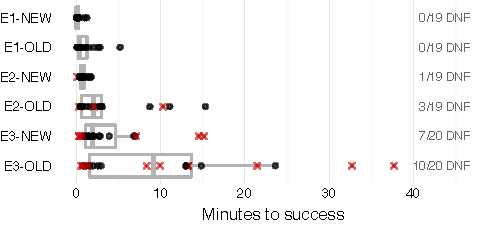
\includegraphics{time_to_success_active_clamped}
\caption{
Only a small fraction of the time was used to configure bridges and proxies.
Non-finishing participants' active time was computed by
subtracting the amount of time spent on the progress screen from the 
their assigned completion time of 40:08.
}
\label{fig:time_to_success_active_clamped}
\end{figure}

%things to keep in mind
We believe that configuration time is a meaningful metric because 1) bootstrapping can dominate measurements for users do not need much time to configure their connection (E1 participants), and 2) many errors do not interrupt the connection attempt and cause many users to wait a long time before they manually cancel the connection to try again. This is metric is not perfect though, since it does not reflect how some participants actively searched for help in another browser rather than passively waiting for their connections to work. 

%configuration time and version
Our interface changes had a significant impact in reducing configuration time (one-tailed Mann--Whitney; $Z = -3.28$, $p = 0.000516$, $r = 0.307$). That is, the differences in mean configuration times in E1-NEW vs E1-OLD and E2-NEW vs E2-OLD and E3-NEW vs E3-OLD is likely not due to random chance. We used a one-tailed Mann--Whitney test because the distribution of configuration times was also 1) right-censored and 2) non-normal and heavily right tailed, due to being an artifact of completion time. 

\subsection{Usability of Tor Launcher} 
We confirmed our observations from our qualitative user test and find that participants wait the progress screen for a long time, spend time configuring proxies when they did not need to, and do not know what to do if the recommended bridge doesn't work. 

From our measurements, we find that 63\% (72 of 114) of first attempts to connect failed and 79\% (363 of 458) of total attempts to connect failed. Users average over 3 minutes if they needed a bridge and averaging over 20 minutes if they needed a meek or custom bridge. 

Ideally, almost all users should be able to configure the necessary or optional network components and connect to Tor within a few minutes. Neither the Tor Browser's 5.0.3 Tor Launcher GUI or our redesigned Tor Launcher GUI meets this goal. 

\section{Recommendations}
\label{sec:recommendations}
We offer some suggestions based on what we learned: \\

\begin{itemize}
\item {\bfseries Hide the proxy configuration screen and less-used transports.} None of our participants connected using flashproxy, fte, fte-ipv6, or scramblesuit transport bridges. Hiding infrequently used options will help users make better choices.
\item {\bfseries Discourage users from configuring optional components.} Many participants configured proxies and bridges that they did not need. Add more explicit guidance on when to use them.
\item {\bfseries Redirect to relevant screens on error.} For instance, redirect users to the bridge screen if the bridge failed instead of requiring users to do so.
\item {\bfseries Take advantage of the progress screen.} Participants spent a majority of their time here. This time could be used to inform them of their bridge and proxy settings, educate users about what Tor does, or introduce Tor Browser.
\end{itemize}

While we believe that adopting our design faithfully will save users time. But since we did not test our design changes independently, we cannot (and do not) claim the effects each change. Alternative designs may be better solutions. 

\section{Limitations}
\label{sec:limitations}
We did not study international users, or the interface in languages other than English. All of our participants were from the United States and were instructed to interact with the English version of Tor Browser.

Participants in a laboratory setting may alter their behavior due to their awareness of being observed~\cite{mccarney2007hawthorne}. Our participants were likely motivated differently compared to real users, but we believe that they were likely overmotivated because they were being observed and receiving a monetary reward. If true, this makes our results a conservative estimate of the usability problems. 

Since the configuration interfaces in simulated environments, we cannot claim how difficult it would be for a user to connect to Tor in a certain country or how much our redesigned interface would help those users.  

Our experiment did not directly test advanced tasks such as configuring a proxy or a custom bridge. From observing  users, we suspect they struggle with these tasks. 

We only tested the interface with Windows machines.
The interface leverages the native operating system's styling and elements, making the configuration interface on Windows look slightly different from the OS~X or Linux equivalents. We acknowledge that participants' unfamiliarity with Windows may have affected our experiment, but we believe that this affected all experimental conditions minorly and equally.  

\section{Related Work}
\label{sec:related} 
% intro to usable security 
The difference between a poor interface and a good interface can influence users’ ability to perform tasks securely~\cite{payne2008brief}. Usable security aims to improve the security of a system by designing with the user in mind. This involves informing users about the system, communicating risks in a way that is understandable, clarifying what the security requirements are, and providing guidance with technical tasks~\cite{adams1999users}. Our work contributes to the body of usable security by evaluating Tor Browser, which is an anonymity and censorship circumvention software that requires user interaction. Other usable security research explores on a variety of security software or features, such as email encryption sofware ~\cite{whitten1999johnny}\cite{garfinkel2005johnny}, authentication methods~\cite{morris1979password}\cite{dhamija2000deja}\cite{suo2005graphical}, web indicators~\cite{dhamija2006phishing}\cite{akhawe2013alice}, and security warnings ~\cite{schechter2007emperor}\cite{egelman2008you}. 

Usability inspection methods~\cite{nielsen1994usability} are used to define usability problems in an interface. We
used a cognitive walkthrough~\cite{wharton1994cognitive}\cite{cognitive-walkthrough} to evaluate our interface. Other inspection methods include heuristic evaluation, pluralistic walkthrough and feature inspection~\cite{inspection}.  

We used usability lab studies (one-on-one experiments with a given a set of scenarios and tasks for a specific use of  a product or service) and usability benchmarking (tightly scripted usability studies are performed with many participants used to collect measures of performance) to get qualitative and quantitative behavioral data about Tor Launcher's GUI~\cite{krol2016towards}. There are other ways to collect behavioral data as well, such as eye tracking, clickstream analysis and AB testing. These are in contrast with a variety of user experience research methods that collect qualitative or quantitative attitudinal data, such as focus group, camera studies, and product surveys~\cite{ux-methods}. We performed interviews after our lab study, but we mostly used these interviews to verify our behavioral observations rather than to draw conclusions about what people thought about their experience. 
 
User-centered design improves the usability of software by accounting for user factors. 
Some work we found especially relevant to improving the usability of Tor Browser were
Yee et~al.'s starting points for reasoning about security from
a user-centered perspective and principles for secure interaction design~\cite{yee2002user},  
Molich et~al.'s examination of  common problems in human-computer dialogue design~\cite{molich1990improving}, and Egelman et~al's examination of user tolerance of security delays~\cite{egelmanplease}.

% Previous Tor studies 
Our work uniquely contributes to Tor by examining the usability of the configuration interface.  
Previous usability studies on Tor have focused on installation and use. Norcie et~al.~\cite{norcie2012eliminating} performed a 25-user test of Tor Browser and found that 64\% of users were unable complete installation or browsing tasks. Fabian et~al.~\cite{fabian2010privately} discussed how added latency benefits anonymity~\cite{dingledine2009performance} but reduces usability. They quantified how the difference in latency causes frustration and decreases adoption. Clark et~al.~\cite{clark2007usability} performed a cognitive walkthrough of Tor Browser deployment options (Vidalia, Privoxy, Torbutton, and FoxyProxy) and found that none were satisfactory from a usability perspective. They highlight the best aspects of each tool and offer usability improvements. We do not know of any published usability evaluations of
Tor Browser the 3.5 series in 2013, which introduced radical UI changes~\cite{torbrowser-35}.
Lee and Fifield~\cite{uxsprint} ran an informal UX sprint that recruited 5 users to install and use Tor Browser tp observe their behavior. This uncovered some usability issues~\cite{uxsprint2015-tickets} and caused UI changes in Tor Browser version~4.5.

\section{Conclusion} 
\label{sec:conclusion}
We believe that an interface is usable if a new user can to identify what to do, knows if and when they do the right thing in the process, and can accomplish the required tasks. Tor Browser 5.0.3's configuration interface does not meet these requirements. We qualified where the interface is not usable with user observations and quantified how unusable the interface is with user interaction logs. We believe that our recommended hanges will will help users connect to Tor in censored environments, but encourage discussion about alternative ways to configure a connection that would be easier for users. 

%proof that user testing is important and general advice to for more research on Tor
Tor Browser version~4.5 incorporated changes to Tor Launcher based on our work <redacted Tor blog post here; it was authored by one of the authors of this paper>. We also talked to Tor developers about ways to automate the bootstrapping process to Tor. We encourage user testing for Tor applications to provide user insight into products that do not collect user data. We found the use of simulated censorship environments were especially helpful in running our experiments, due to their reproducibility, stability, and simplicity.

\section {Experiment Artifacts} 
Due to space constraints, we could not include many of our experiment artifacts. This includes the experiment setup and teardown code, firewall rules that simulated censorship environments, interview transcriptions from the qualitative user study, logs from our instrumented configuration interfaces, and videos of users attempting to connect to Tor through the configuration interface. We urge you to check out the project repository: \\

\noindent <redacted url>
%\noindent \url{https://github.com/lindanlee/circumvention-ux-tor}

\section {Acknowledgments}
Many generous people helped us along the way. <Redacted> assisted with testing our setup and teardown scripts, offered recruitment services, and allowed us to run experiments after <redacted lab>'s hours. <Redacted> and <redacted> were instrumental during the design process, as they helped me iterate through many not-so-great ideas.  <Redacted> and <redacted> provided me with insider insight into the design decisions made at Tor.
% Rowilma del Castillo. Nima Fatemi and Isabela Bagueros.  Georg Koppen and the Tor UX team.

\bibliographystyle{abbrv}
\bibliography{pets2017-paper.bib}

\appendix

\section{Success and Error States in Tor Launcher 5.0.3} 
\label{states} 
Tor Launcher 5.0.3's end states corresponding to Figure~\ref{fig:digraph}. E\# and $\mbox{e\#}^\prime$ are equivalent, but $\mbox{e\#}^\prime$ uses a bridge while e\# does not. \\

\noindent success states: 
\begin{itemize}
\item s0: no bridge no proxy
\item s1: valid bridge, no proxy
\item s2: valid bridge and valid proxy (blank port)
\item s3: valid bridge and valid proxy (specified port)
\end{itemize}

error states:
\begin{itemize} 
\item e0: need a bridge or proxy
\item e1: hardcoded bridge blocked
\item e2: custom bridge: field left blank
\item e3: custom bridge: syntax error
\item e4: custom bridge: invalid address
\item e5: custom bridge blocked
\item e6: proxy type is not selected
\item e7: proxy: ip address left blank
\item e8: proxy: syntax error
\item e9: proxy: invalid IP address, blank port
\item e10: proxy: invalid IP address, good port
\item e11: proxy: invalid IP address, bad port
\item e12: proxy: valid IP address, bad port
\item e13: proxy: valid IP address, blank port
\end{itemize} 

Same inputs can lead to different end states. Tor Launcher will connect to a proxy successfully with the port left blank if the proxy uses port 80 (s2) but will not if the proxy uses another port (e12). 

\section{Qualitative User Study Recruitment Posting} 
\label{qualitative-recruitment}
We are recruiting participants for an in-person research study at <redacted>. %the University of California, Berkeley. 
You will need to come in to our lab and perform tasks on a computer for an hour or less. You will be compensated \$30 for participating. 
No special knowledge and no technical experience is required. If you are interested, fill out the survey at \textit{<survey link>}. 

\section{Qualitative User Study Prescreening Survey} 
\label{qualitative-prescreening}
We are recruiting participants for an in-person research study at the <redacted>. %University of California, Berkeley. 
You will need to come in to our lab and perform tasks on a computer for an hour or less. You will be compensated \$30 for participating. No special knowledge and no technical experience is required.\\

\begin{enumerate}
\item{Please select when you are available. We will assign you an hour experiment time slot during one of those times.}
\item{I am able to provide my own transportation to the <redacted> %University of California, Berkeley 
campus.}
\item{Thank you for your interest! Please provide an email address where we can contact you to share more logistical details.}
\item{we are looking for a very small number of participants, so unfortunately, we may not be able to accommodate everyone who applies. Would you like us to let you know about future opportunities?}
\item{What is your gender?}
\item{What is your age?}
\item{Please select your highest completed (or current) level of education.}
\item{What is your occupation?} 
\item{Do you speak any languages other than English fluently?}
\item{If you have a personal computer, what kind do you use?}
\item{Which of the following terms have you heard of? \textit{<answer choices: a checkboxlist of the the following terms: malware, proxy services, phishing, SSL, X.511 certificates, Tor>}}
\item{How often do you use the following software or features? \textit{<answer choices: a grid of radio buttons. Software/features (rows): HTTPS on web pages, proxies or other censorship circumvention tools, virtual private networks (VPN), file or whole-disk encryption, anonymity systems (e.g., Tor), email encryption (e.g., PGP), chat or instant messaging encryption, voice communication encryption. Frequency (columns): never, less than once a month, a few times a month, several times a week, daily.>}}
\end{enumerate}
Thank you for filling out this form. You are now done!

\section{Qualitative User Study Introduction Script} 
\label{qualitative-script} 
Imagine you live in an oppressive country that censors part of the Internet. We have simulated this in the laboratory by blocking certain websites and services.  The purpose of this experiment is to evaluate the use of Tor browser, which is a browser that can circumvent censorship and let you visit blocked websites. Currently, torproject is blocked (you can check this by going to torproject.org on a standard browser, like Firefox, Chrome, or Internet Explorer). 

To circumvent censorship successfully, you will need to set up Tor browser correctly and use it to get to Wikipedia. If you are able to reach the website, then you know that you have successfully circumvented censorship. Fill out the question on the worksheet. This isn't intended to be hard, just write what you see. We want to just check you saw the website. 

Before you start, do you have any questions about what you are asked to do? 

\section{Qualitative Study Worksheet Text} 
\label{participant-worksheet}
Imagine you live in an oppressive country that censors part of the Internet. We have simulated this in the laboratory by blocking certain websites and services. The purpose of this experiment is to evaluate the use of Tor browser, which is a browser that can circumvent censorship and let you visit blocked websites. For instance, www.torproject.org is blocked. Check this by going to the site on a standard browser, like Firefox, Chrome, or Internet Explorer. It will fail to load, when you can visit other sites.

To complete this worksheet, you will need to set up Tor browser (on your desktop) correctly and use it to get to blocked site. If you can visit wikipedia, then you know that you have successfully circumvented censorship.

\section{Post-Experiment Standard Interview Questions}
\label{interview-questions}
We asked our participants these questions after they were given time to configure Tor Browser. \\

\begin{enumerate}
\item{Can you talk us through what you did along with what you were thinking at the time?}
\item{What was most challenging part of connecting?}
\item{Were there any unfamiliar terms?}
\item{How did you decide which options to choose?}
\item{What did you think about using Tor?}
\item{What is one change you would recommend?} 
\item{Did you need any additional information?} 
\end{enumerate}  

In addition to these questions, we asked our participants about specific questions based on their observation, usually regarding a specific choice in action, a particular screen they seemed stuck on, and any errors they encountered during the configuration process. 

\section{Qualitative Testing Observations}
\label{summary}
We summarize of each participant's session.

%E1: P2, P3, P4, P9, P10
%E2: P7, P8, P11, P12, P13
%E3: P1, P5, P6, P14, P15, P16

% re-watched the videos and get the exact times. 
%https://github.com/lindanlee/PETS2017-paper/tree/master/sessions/pre/videos

\subsubsection{E1} 
In E1, any connection to Tor worked. Configuring bridges and proxies was optional.  
Observations in E1: 

%P9 (regular): E1 (0:39; 4:49 to 5:28)
\pquote{P1 (new user, direct, 0:39)}{They connected directly.}

%P2(regular): E1 (1:20, 0:22 to 1:42) 
\pquote{P2 (new user, direct, 1:20)}{They spent time reading the text on the start screen, and connected directly because they were intimidated by the other option.}

%P3(regular): E1 (N/A; 5:47 to 6:26) 
\pquote{P3 (new user, obfs3, 1:39)}{They connected with the recommended bridge. They were also going to use a proxy, but decided not to when they saw the proxy input fields.}

%P4(regular): E1 (8:56, 7:22 to 16:18)
\pquote{P4 (new user, obfs4, 8:56)}{They chose the recommended bridge and then tried to configure a proxy. After not being able to fill out the proxy input fields, they started over and connected with an obfs4 bridge. Note that they did not try connecting with the obfs3 bridge, which would have worked.}

%P10 (has used Tor before): E1 (1:02; 0:13 to 1:15)
\pquote{P5 (previous Tor user, obfs3, 1:02)}{They connected with the recommended bridge.}

Participants in E1 were able to connect to Tor, but most were unsure if their actions were correct. Three of the five participants unnecessarily configured bridges. 

\subsubsection{E2} 
In E2, a bridge was required to connect. Any of the hardcoded bridges from the dropdown menu, as well as any custom bridges acquired out of band would work. Configuring a proxy was optional.
Observations in E2: 

%P7 (heard of Tor): E2 (4:04; 0:29 to 4:33) 
\pquote{P6 (new user, obfs3, 4:04)}{They tried connecting directly. After watching the progress bar not make any progress for a couple minutes, and gave up on the direct connection. Then they connected with the recommended bridge.}

%P13 (regular): E2 (7:48; 0:34 to 9:22) 
\pquote{P7 (new user, obfs3, 9:22)}{They tried connecting directly. They restarted Tor Launcher and tried to connect directly again---and repeated this two more times. On the fourth restart, they tried to configure a proxy, but gave up. On the fifth restart, they connected using the recommended bridge.}

%P12 (regular): E2 (10:40; 0:46 to 11:26)
\pquote{P8 (new user, direct, 10:40)}{They tried connecting directly. After waiting a couple minutes, they figured that did not work and looked at proxy settings. But after looking at the settings and being intimidated, they tried connecting directly again. Then, they tried to configure a proxy, and gave up. They tried connecting directly again, which worked unexpectedly. They found a bug in our setup that we fixed for the later experiment. E2 required a bridge to connect, but new public relays came online after we ran our firewall rules and they were able to connect using those new relays. }

%P11 (used Tor before): E2 (~3:00; 1:05 to 5:13)
\pquote{P9 (previous Tor user, obfs3, 4:08)}{They tried connecting directly. And they tried connecting directly through a different user path by answering no to bridge and proxy questions in the interface, connecting from the proxy screen. Then, they connected using the recommended bridge.}

%P8 (used Tor): E2 (clock drift mission impossible, 1:38 to 7:20) 
\pquote{P10 (previous Tor user, failed to connect)}{They tried a direct connection. Then, they tried a connection with the recommended bridge, which should have worked. However, our setup experienced a clock drift. Tor does not allow connections with bad clocks. They spent the rest of their time trying different bridges and proxies in vain (Figure~\ref{fig:proxy-attempt}). This participant tried the most attempts to connect to Tor, using a variety of bridges and proxies.}

Participants in E2 tried a direct connection to Tor before {\it eventually} connecting with the recommended bridge.
They spent a fair amount of time waiting before determining that connections failed. Some stated that they connected directly because the interface says that it would work in ``most situations'' (Figure~\ref{fig:old-first}). Our participants did not know if they needed bridges or proxies, so they only tried to configure one when the direct connection failed. Since they did not know whether they needed a bridge or proxy, they often tried to configure proxies when they did not need one and should have configured bridges instead.  

\subsubsection{E3}
In E3, a bridge was required to connect. Most of the hardcoded bridges in the dropdown menu do not work, with the exception of meek-amazon, meek-azure, and meek-google. Custom bridges can also work. Configuring a proxy was optional.
Observations in E3: 

\begin{figure}[t]
\centering
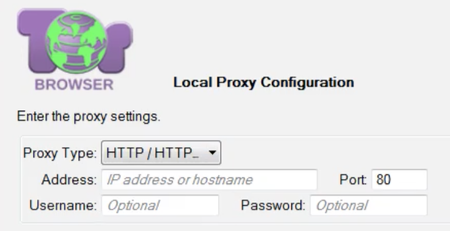
\includegraphics[width=0.5\textwidth]{P8-proxy-attempt.png}
\caption{
Proxies were not necessary to connect to Tor, but many spent time trying to configure one when they couldn't connect. None succeeded. Here, we show P10's unsuccessful attempt. 
}
\label{fig:proxy-attempt}
\end{figure}

%P14 (regular): E3 FAIL
\pquote{P11 (new user, failed to connect)}{They tried connecting directly, and then with the recommended bridge. Then, they retried connecting directly and retried connecting using the recommended bridge. After that, the participant spent the rest of their time trying to configure a proxy and retrying connections with the recommended bridge.}

%P15 (regular): E3 FAIL
\pquote{P12 (new user, failed to connect)}{They tried connecting with the recommended bridge. They decided that they need a proxy along with the recommended bridge, and spent the rest of their time trying to configure a proxy.}

%P16: E3 (regular) FAIL
\pquote{P13 (new user, failed to connect)}{They tried connecting directly, and then with the recommended bridge. They retried connecting with the recommended bridge. When that didn't work, they tried to configure a proxy. Then, they gave up on the task entirely.}

%P6 (heard of Tor): E3 (26:48; 0:18 to 27:06) 
\pquote{P14 (new user, meek-google, 26:48)}{They tried a direct connection by answering no to bridge and proxy questions. After waiting a while, they canceled the connection and tried connecting with the recommended bridge. They retried connecting with the recommended bridge two more times, then tried to connect with a flashproxy bridge, an obfs4 bridge, a scramblesuit bridge. After retrying the recommended bridge again, they made a connection using a meek-google bridge.}

%P1 (heard of tor before): E3 (~7:31, 0:51 to 8:22) 
\pquote{P15 (new user, meek-azure, 7:31)}{They tried connecting directly, and then with the recommended bridge. After that, they tried a connection using a meek-azure bridge, but gave up after before it could connect. They went back to the first screen~\ref{fig:old-first} and clicked connect, which made a connection using meek-azure bridge. The connect button makes a connection to Tor with the toggled settings in the interface. When the interface is initialized to not use a bridge or proxy, clicking connect on the first page starts a direct connection. But since the participant had chosen a meek-azure bridge, the connect button made a connection to a meek-azure bridge, even though the text in the first screen says that they will ``connect directly.'' Because of this, the participant thought they made a direct connection. Although they succeeded in connecting to Tor, they did not realize what they had done or why connecting to a meek-azure bridge worked. They chose that bridge at random.}

%P5 (has used tor before): E3 (22:06; 0:00 to 22:06)
\pquote{P16 (previous Tor user, custom bridge, 22:06)}{They tried and retried connecting directly, then they tried connecting with the recommended bridge. After briefly looking at error messages the system log, they retried connecting directly two more times. After trying to configure a proxy for a while, they instead decided not to use one and tried connecting with a meek-google bridge, which would have worked. But  due to a bug in the progress bar that prevents it from updating correctly on subsequent attempts, they gave up before it could connect. They made a connection with the custom bridge by following the instructions from the bridge help button (they created a throwaway email account, emailed the bridge responder with poor syntax and did not get a response, emailed the bridge responder again with correct syntax and got a response, and then typed in the bridge information into the custom bridge field).}

Participants in E3 also generally tried a direct connection to Tor. They did not know if they needed a bridge or proxy, and like the participants in E2, only configured them when the direct connection failed. But even if the participants were able to figure out that they needed a bridge and not a proxy, the recommended bridge will not work. Of the participants that failed, they all tried the recommended bridge but not any others. The participants that did manage to connect to Tor did not know which bridges worked and which ones did not, or which ones to try next in case the recommended one failed. P14 brute forced options until something worked, P15 did not think that they used a bridge, and P16 gave up on a hardcoded bridge that would have worked and used a custom bridge instead.

\section{Alternative Approaches} 
\label{alternatives}
{\color {red}
\begin{itemize} 
\item{\bfseries Suggest bridges based on country.} Give users information about which bridges would work in their country. one way to do this is to show a list of countries with a corresponding recommended configuration. This requires developers to maintain a list of suggestions and that the users trust the suggestions. 
\item{\bfseries Ask users about their risk.} If they answer that they are sensitive about having a network adversary possibly know that they are using Tor, direct users to connect to a secret relay that is not publicly associated with Tor, using transport that obfuscates their connection. If users are not sensitive, let them configure their own bridges and proxies. 
\item{\bfseries Ask users if they know what to do.} If they know, offer the option to manually configure bridges and proxies. If they do not know, give suggestions on what to do next or automate the process for them somehow. This requires users to answer honestly to the question and to trust the suggestions given. 
\item{\bfseries Automate naively.} Have the interface automatically try configurations that would most likely work, in order (i.e. a direct connection, then an obfs3 connection without a proxy, then an meek bridge connection with out a proxy). This is what most users would ideally do anyway. However, this method leaks to network eavesdroppers that the user is using Tor without the user's awareness. 
\item {\bfseries Automate naively after users fail.} Let users try to configure bridges and proxies. If they fail, then a network eavesdropper already knows that the user is trying to connect to Tor. We believe there is negligible added risk to naively automate the connection. 
\item{\bfseries Automate in a smart way.} The interface first detects proxy settings and uses them, if any. Then it automatically connects to some secret bridges that will always work, which assign the user an entry relay that works based on their location. This requires having an invincible set of high-bandwidth bridges that work for every single user around the world.  
\end{itemize}
We believe that these ideas can significantly help users connect to Tor.
}

\section{Quantitative User Study Recruitment Posting}
\label{quantitative-recruitment}
We are recruiting up to 40 participants for a user study at <redacted>. %UC Berkeley. 
The experiment will involve basic Internet browsing tasks. You are not eligible if you have participated in our previous sessions.\\

\indent Payment: \$30 Amazon gift card\\
\indent Duration: 1 hour \\
\indent Where: <redacted> \\ %Xlab at Hearst Memorial Gymnasium\\

\textit{<list of sessions>}\\

To be eligible, you must be an adult (18 or older). This is to comply with university policies on research. 

If you are interested: 1. Email <redacted> %lnl@berkeley.edu 
with the sessions you are able to attend. We will confirm your participation and assign you a session. 
2. Come to <redacted> %Xlab 
at the appointed time for the experiment.

\section{Quantitative User Study Introduction Script} 
\label{quantitative-script} 
Imagine you live in an oppressive country that censors part of the Internet. We have simulated this in the laboratory by blocking certain websites and services.  The purpose of this experiment is to evaluate the use of Tor browser, which is a browser that can circumvent censorship and let you visit blocked websites. Currently, torproject is blocked (you can check this by going to torproject.org on a standard browser, like Firefox, Chrome, or Internet Explorer). 

To circumvent censorship successfully, you will need to set up Tor browser correctly and use it to get to Wikipedia. Tor is already installed for you. On the desktop, you should see a globe icon that says ``Start Tor Browser.'' If you are able to reach the website, then you know that you have successfully circumvented censorship. Fill out the question on the worksheet. This isn't intended to be hard, just write what you see. We want to just check you saw the website. 

Afterward, we ask you to take a short survey to collect some information about you. The link is also on your worksheet.
We will give you time to complete this task. If you finish early, we ask that you sit at your desk until the remainder of the hour. Since we are recording your screen, we ask that you don't do anything personal afterward, like checking your email.

Before you start, do you have any questions about what you are asked to do? 

\section{Quantitative User Study Worksheet Text} 
\label{summative-worksheet}
Imagine you live in an oppressive country that censors part of the Internet. We have simulated this in the laboratory by blocking certain websites and services.

The purpose of this experiment is to evaluate the use of Tor browser, which is a browser that can circumvent censorship and let you visit blocked websites. For instance, www.torproject.org is blocked. Check this by going to the site on a standard browser, like Firefox, Chrome, or Internet Explorer. It will fail to load, when you can visit other sites.

To complete this worksheet, you will need to set up Tor browser (on your desktop) correctly and use it to get to blocked site. If you can visit wikipedia, then you know that you have successfully circumvented censorship.

1. Visit Wikipedia’s main page (\url{https://en.wikipedia.org/wiki/Main\_Page}). What is the topic of today’s selected article? 

2. After you have completed the tasks, fill out this survey: http://bit.ly/tor-survey 


\section{Quantitative User Study Exit Survey} 
\label{quantitative-exit-survey}
We'd like to know more about you.  All of your answers will be stored separately from any identifying information in order to protect your confidentiality.

This survey is part of a research project being conducted by the <redacted>. %University of California, Berkeley. 
If you have any questions about your rights or treatment as a research participant in this study, please contact the <redacted>'s %University of California at Berkeley's 
Committee for Protection of Human Subjects at 510-642-7461, or email 
<redacted>. %subjects@berkeley.edu. 
If you agree to participate, please click Next below.\\

\begin{enumerate}
\item{What is your participant ID? (This can be found on the sticker on the left hand corner of the desk you are currently sitting at.)}
\item{What is your gender?}
\item{What is your age?}
\item{Please select your highest completed (or current) level of education}.
\item{What is your current occupation?}  
\end{enumerate}

Thank you for participating in our experiment. You are now done! Please sit at your desk for the remainder of the experiment. Our researchers will formally announce the end of the experiment. 


\end{document}
